\documentclass[12pt]{article}

\usepackage{sbc/sbc-template}
\usepackage{graphicx,url}
\usepackage[brazil]{babel}
\usepackage[utf8]{inputenc}

\sloppy

% Metadata
\title{Modelagem de um cruzamento de quatro semáforos utilizando Redes Coloridas de Petri}
\author{João Pedro Pereira Lemos\inst{1}}
\address{Instituto Federal de Educação, Ciência e Tecnologia do Estado do Ceará (IFCE)
  \email{joao.pedro.pereira62@aluno.ifce.edu.br}
}

\begin{document} 

\maketitle

% Abstract
\begin{abstract}
  The article proposes a simplified approach to modeling a road intersection, focusing exclusively on the interaction between the four traffic lights present.
Using Colored Petri Nets as a modeling framework, the study seeks to provide a clear representation of the traffic control dynamics at the intersection.
By focusing on communication between traffic lights, the article seeks to simplify the understanding of the system, highlighting the essential aspects for a robust understanding of the flow of vehicles at the intersection.
This targeted approach aims to provide a solid foundation for future analysis and optimization, contributing to the development of more efficient and adaptable traffic control systems.
\end{abstract}
     
\begin{resumo}
  O artigo propõe uma abordagem simplificada para a modelagem de um cruzamento viário, focando exclusivamente na interação entre os quatro semáforos presentes.
Utilizando Redes Coloridas de Petri como estrutura de modelagem, o estudo busca oferecer uma representação clara da dinâmica de controle de tráfego no cruzamento.
Ao se concentrar na comunicação entre os semáforos, o artigo busca simplificar o entendimento do sistema, destacando os aspectos essenciais para uma compreensão robusta do fluxo de veículos no cruzamento.
Essa abordagem direcionada visa fornecer uma base sólida para futuras análises e otimizações, contribuindo para o desenvolvimento de sistemas de controle de tráfego mais eficientes e adaptáveis.
\end{resumo}


% Introduction
\section{Introdução}

Em meio ao contínuo crescimento urbano e à expansão das redes viárias, a eficiente gestão do tráfego torna-se imprescindível para garantir a fluidez e a segurança no transporte urbano.
Nesse contexto, os cruzamentos viários desempenham um papel crucial, representando pontos críticos onde a coordenação entre os semáforos se torna essencial para otimizar o fluxo de veículos.
Este artigo se concentra na modelagem de um cruzamento composto por quatro semáforos, utilizando Redes Coloridas de Petri.

As Redes Coloridas de Petri, uma extensão das tradicionais Redes de Petri, emergem como uma ferramenta poderosa para representar sistemas dinâmicos e distribuídos.
Ao aplicar esta metodologia à modelagem de cruzamentos viários, buscamos proporcionar uma compreensão mais aprofundada da interação entre os semáforos, concentrando-nos exclusivamente na comunicação entre esses elementos-chave.
A simplificação deliberada do escopo do estudo visa oferecer uma visão clara e concisa, permitindo uma análise mais eficaz da dinâmica de controle de tráfego no cruzamento.

Exploraremos, ao longo deste artigo, a aplicação prática das Redes Coloridas de Petri na modelagem de sistemas de tráfego, observando o controle de quatro semáforos em um cruzamento.
Ao fazer isso, almejamos contribuir para o avanço da compreensão teórica e prática dos sistemas de controle de tráfego, abrindo caminho para estratégias mais eficientes e adaptáveis na gestão do tráfego urbano.


% Foundation
\section{Fundamentação teórica}

A modelagem de sistemas complexos, como cruzamentos viários, requerem abordagens analíticas robustas que possam capturar de modo eficiente as dinâmicas envolvidas.
As Redes de Petri, introduzidas por Carl Adam Petri na década de 60, fornecem uma estrutura gráfica poderosa para a representação e análise de sistemas dinâmicos e concorrentes.

Uma Rede de Petri é composta por lugares, transições, tokens e arcos direcionados.
Os lugares representam estados do sistema, as transições indicam eventos ou ações, os tokens denotam a presença de recursos ou condições, e os arcos modelam as relações e transições permitidas~\cite{petri-nets-paper}.

As Redes Coloridas de Petri são uma extensão desta teoria que incorporam atributos coloridos para enriquecer a representação de informações e estados do sistema.
A adição de cores permite uma modelagem mais expressiva, possibilitando a análise de sistemas com características mais intrínsecas e variáveis~\cite{colored-petri-nets-book}.
A utilização de Redes Coloridas de Petri é relevante em contextos onde a representação precisa de múltiplos estados do sistema é crucial, como é o caso da dinâmica de semáforos em um cruzamento.

Um dos pilares fundamentais das Redes Coloridas de Petri é a capacidade de representar eventos concorrentes e a evolução temporal de um sistema.
Este formalismo fornece uma base sólida para a análise de sistemas dinâmicos complexos, incluindo aqueles encontrados em aplicações de controle de tráfego~\cite{petri-nets-applications-article}.

Ao integrar os princípios fundamentais das Redes Coloridas de Petri com a dinâmica específica de cruzamentos viários que envolvem quatro semáforos, este estudo visa contribuir para o avanço da teoria e prática no campo do controle de tráfego, promovendo estratégias mais eficazes e adaptáveis na gestão do tráfego urbano.


% Methodology
\section{Metodologia}

Para atingir o objetivo deste artigo, criou-se uma Rede de Petri para simular um cruzamento com quatro semáforos.
A ferramenta CPN IDE foi utilizada para criar e simular a Rede de Petri~\cite{cpn-ide}.
Cada semáforo apresenta três estados possíveis: fechado (indicado pela cor vermelha), próximo ao fechamento (indicado pela cor amarela) e aberto (indicado pela cor verde).
Os semáforos foram dispostos, com dois na direção horizontal e outros dois na direção vertical.

A Figura~\ref{fig:traffic_light} apresenta a modelagem de um semáforo por meio de uma Rede Colorida de Petri.
Nesse modelo, cada lugar representa um dos estados possíveis do semáforo: fechado, próximo ao fechamento e aberto.
Todos os lugares são do tipo INT\@.
Inicialmente, cada semáforo inicia com duas fichas no estado fechado.
Três transições foram definidas: uma que move uma ficha do lugar vermelho para o verde, outra que move uma ficha do verde para o amarelo e, por último, uma que move uma ficha do amarelo para o vermelho.
Os arcos sempre consomem duas fichas.

\clearpage

\begin{figure}[ht]
	\centering
	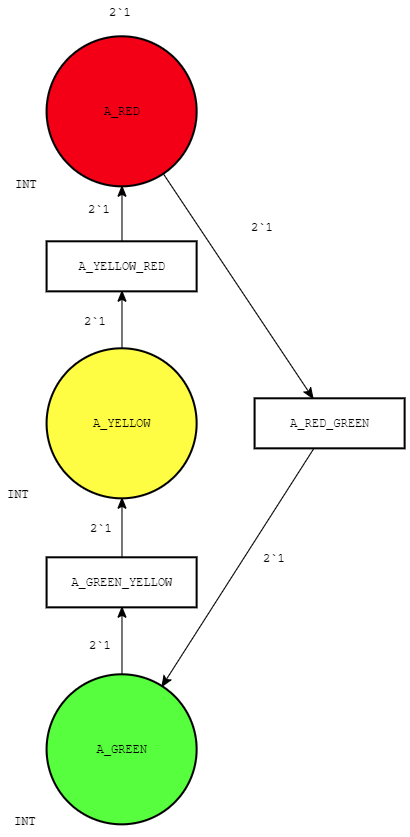
\includegraphics[width=0.55\textwidth]{images/traffic_light.png}
	\caption{Modelagem de um semáforo utilizando uma Rede Colorida de Petri}
    \label{fig:traffic_light}
\end{figure}

Para integrar-se com outros semáforos, foi necessário realizar algumas modificações na rede.
A Figura~\ref{fig:two_traffic_lights} ilustra a modelagem de uma Rede Colorida de Petri que conecta o funcionamento de dois semáforos.
Embora o semáforo em si permaneça inalterado, foram introduzidos novos arcos que vinculam os dois semáforos.

Dois arcos adicionais foram incorporados, consumindo fichas dos lugares vermelhos quando as transições de cada semáforo são acionadas, movendo a ficha do lugar vermelho para o lugar verde no mesmo semáforo.

Adicionalmente, outros dois novos arcos foram introduzidos, inserindo novamente fichas nos lugares vermelhos de cada semáforo no momento em que a transição que move a ficha do lugar amarelo para o lugar vermelho no mesmo semáforo é acionada.

Quando um dos semáforos está no estado aberto, os demais semáforos na rede devem permanecer no estado fechado, com as transições que alteram seus estados desabilitadas.
Os arcos que consomem fichas dos lugares vermelhos consomem apenas uma ficha, assegurando que o lugar vermelho do semáforo mantenha uma ficha, indicando assim o estado fechado.

Quando o semáforo que estava aberto retorna ao estado fechado, as fichas que foram consumidas dos outros semáforos devem ser restituídas.
Dessa forma, o arco que insere fichas nos lugares vermelhos dos semáforos passa a inserir apenas uma ficha, fazendo com que o lugar vermelho do semáforo volte a ter duas fichas, também indicando o estado fechado.

\begin{figure}[ht]
	\centering
	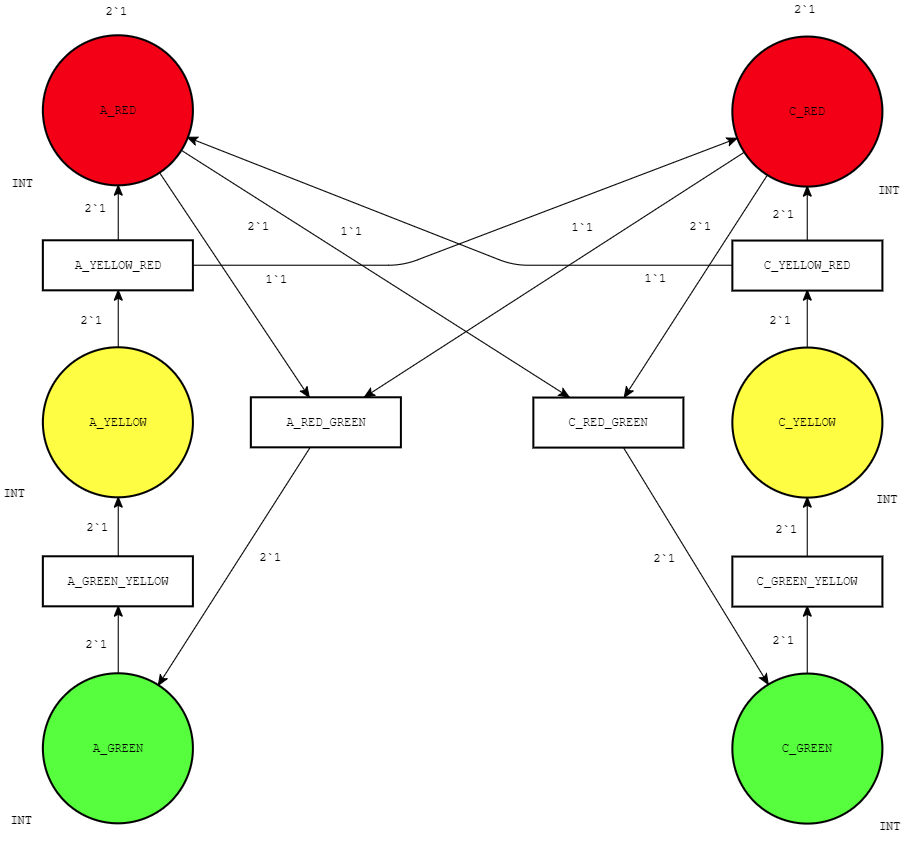
\includegraphics[width=1\textwidth]{images/two_traffic_lights.png}
	\caption{Modelagem da integração de dois semáforos}
    \label{fig:two_traffic_lights}
\end{figure}

Executando as adições correspondentes em cada um dos quatro semáforos, alcançamos a configuração final de nossa rede.
Nesse ponto, ocorre a movimentação consistente de tokens entre todos os semáforos, bem como a sua reposição.
A representação completa desse processo é visualizada na Figura~\ref{fig:full_petri_net}.

\begin{figure}[ht]
	\centering
	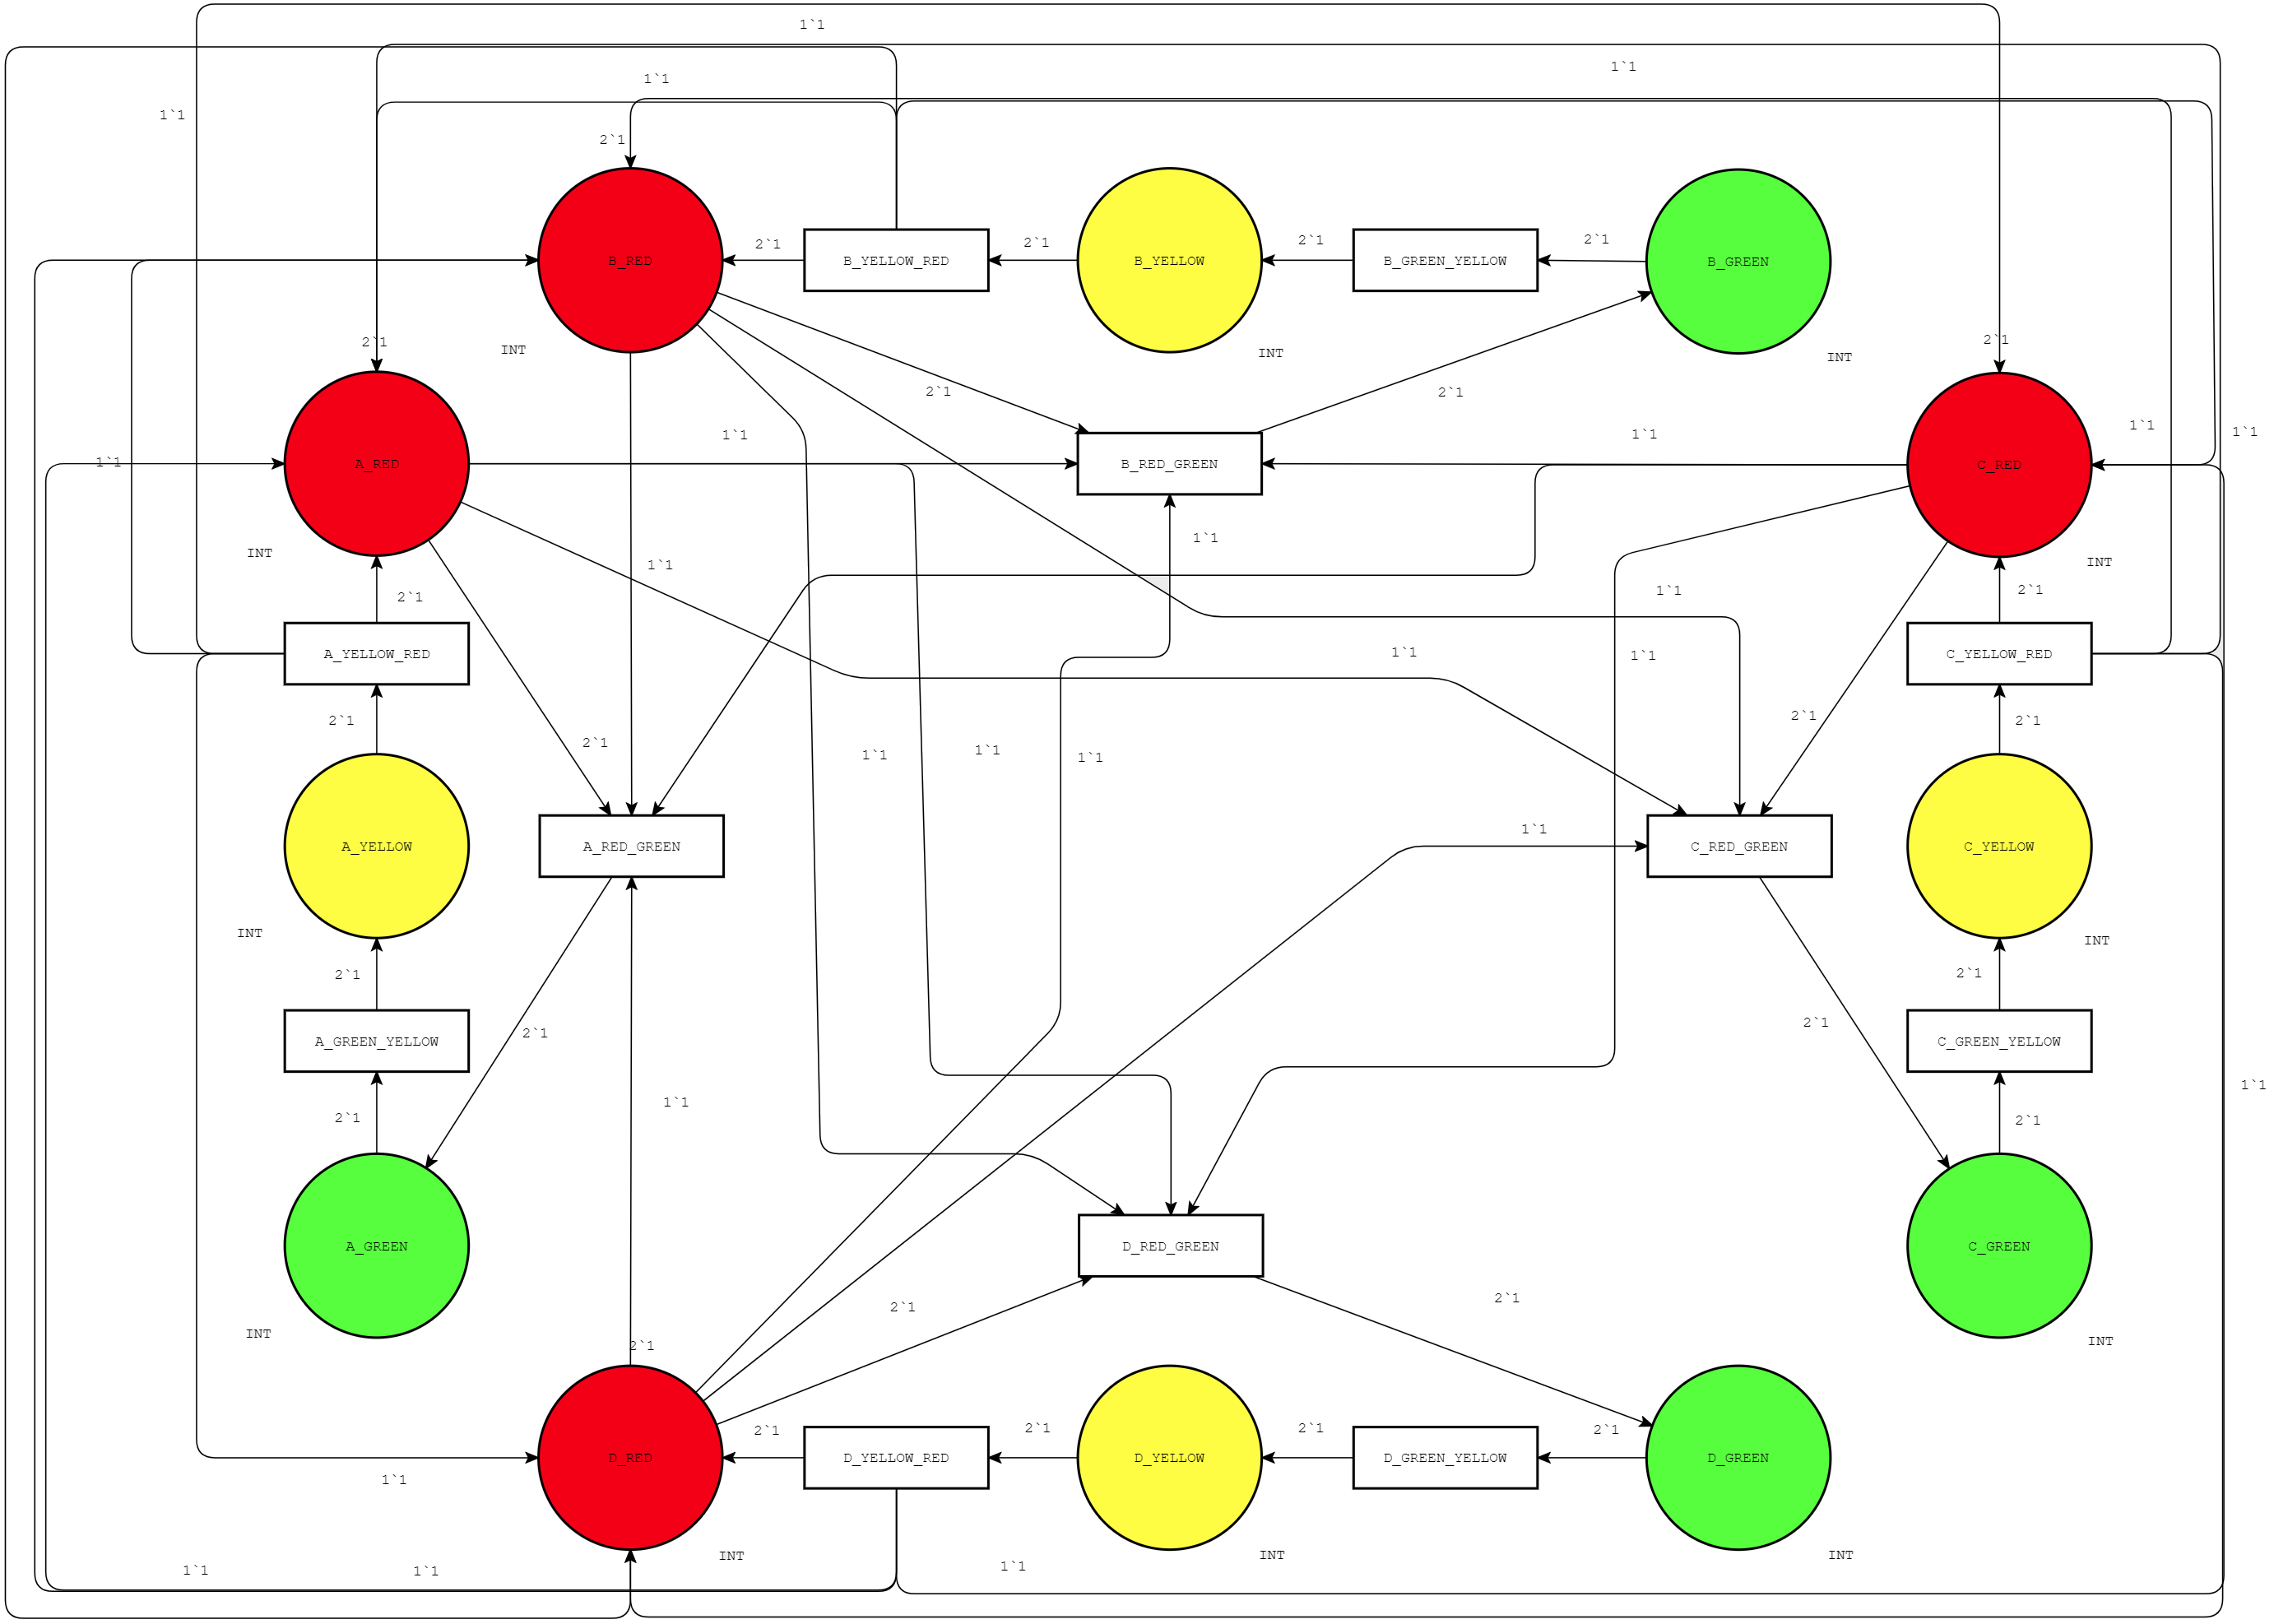
\includegraphics[width=1\textwidth]{images/full_petri_net.png}
	\caption{Modelagem completa do cruzamento de semáforos}
    \label{fig:full_petri_net}
\end{figure}


% Results
\section{Resultados obtidos}

A seguir são apresentados os resultados obtidos.


% Conclusion
\section{Conclusões}

Conclusões do artigo


% Bibliography
\bibliographystyle{sbc/sbc}
\bibliography{sbc/sbc-template}

\end{document}
